\frame{\frametitle{Data Access Services}
\begin{columns}
    \begin{column}{0.6\textwidth}
        \begin{itemize}
            \item Catalog Database (Qserv) to 100 TB range
            \begin{itemize}
                \item Three 30-node clusters operating:
                \begin{itemize}
                    \item NCSA (PDAC): science dataset (Stripe 82 + AllWISE + NEOWISE)
                    \item CC-IN2P3 (2 x dev): synthetic dataset
                \end{itemize}
                \item 30\% DR1 KPM measurements in progress
                \item Jun 2018:
                    \begin{itemize}
                        \item Deployment under Kubernetes
                        \item Data replication and auto-recovery
                        \item Revamped loader/ingest tools
                        \item HSC load
                    \end{itemize}
                \item Dec 2018:
                    \begin{itemize}
                        \item GAIA DR2 load
                    \end{itemize}
            \end{itemize}
        \end{itemize}
    \end{column}
    \begin{column}{0.4\textwidth}
        \begin{center}
            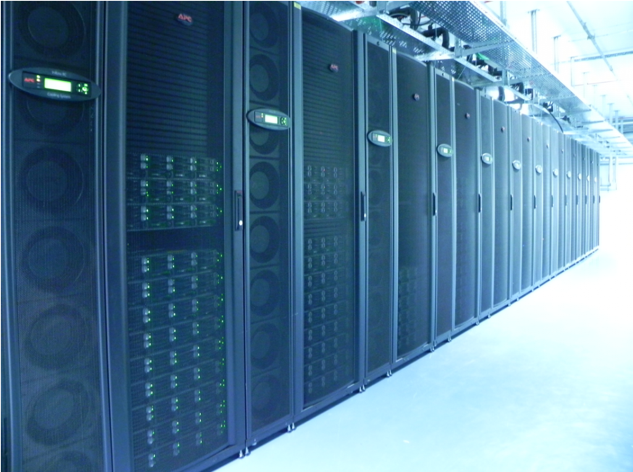
\includegraphics[width=\columnwidth]{figures/qserv-in2p3.png}
        \end{center}
    \end{column}
\end{columns}
}

\frame{\frametitle{Data Access Services}
\begin{columns}
    \begin{column}{0.7\textwidth}
        \begin{itemize}
            \item Web Services for Science Platform -- Standards Orientation\\~
            \begin{itemize}
                \item Bespoke endpoints now being replaced with IVOA compliant services:
                    \begin{itemize}
                        \item TAP/ADQL, SIAv2, SODA, VOspace, UWS
                    \end{itemize}
                \item Standards-oriented metadata:
                    \begin{itemize}
                        \item RegTAP, VOResource, ObsCore, CAOM, UCD
                    \end{itemize}
                \item Jun 2018: Revamped TAP/ADQL query services
                \item Dec 2018: Revamped image cutout and metadata services
            \end{itemize}
        \end{itemize}
    \end{column}
    \begin{column}{.3\textwidth}
        \begin{center}
            
\includegraphics[width=\columnwidth]{figures/ivoa.jpg}
        \end{center}
    \end{column}
\end{columns}
}

\frame{\frametitle{Middleware}
\begin{itemize}
    \item Gen 3 Data Butler and Supertask\\~\

    An object-oriented data archive abstraction (Butler) and workflow infrastructure (Supertask).  Needed cleanup/attention!\\~\
    \begin{itemize}
        \item Working group convened; from scratch in-depth exploration of use cases
        \item New design resulted; scrum team assembled
        \item Jun 2018: support for HSC camera
        \item Dec 2018: replace Gen 2 code throughout DM stack
    \end{itemize}
\end{itemize}
}
